\section{Experiments}
\label{sec:experiments}
% \tk{order: CLEVR + baselines without TL, COG + baseline without TL, Feature Transfer-CLEVR/CoGenT, Temporal Transfer - COG, Reasoning Transfer - CLEVR/CoGenT, Reasoning Transfer-COG}

\begin{figure}[b!]
	\centering
	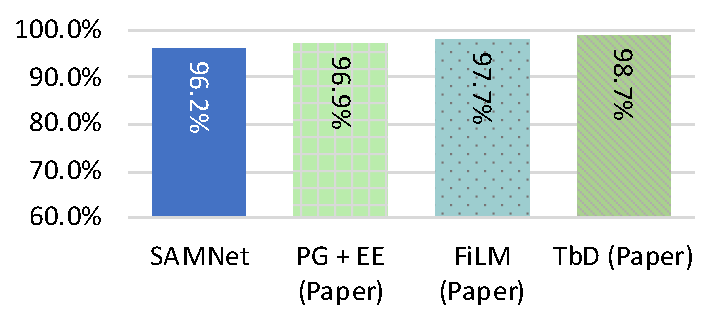
\includegraphics[width=0.5\textwidth]{../img/plots/clevr_baselines.pdf}
	\caption{Comparison of SAMNet to baselines on CLEVR.}
	\label{fig:clevr_baselines}
\end{figure}


We implemented and trained our SAMNet model using MI-Prometheus~\cite{kornuta2018accelerating}, a framework based on PyTorch~\cite{paszke2017automatic}.
We evaluated the model on
the CLEVR dataset~\cite{johnson2017clevr}, a diagnostic dataset for Image Question Answering and on the COG dataset~\cite{yang2018dataset}, a video reasoning~\cite{mogadala2019trends} dataset developed for the purpose of research on relational and temporal reasoning.
We briefly describe both datasets in the following two subsections.
In all experiments, we trained SAMNet using $T = 8$ reasoning steps and external memory with $N = 8$ slots, each storing an array of $d = 128$ floats.
When working with CLEVR, we deactivated SAMNet's external memory and temporal-related modules as they are unnecessary while reasoning about static images.

We start with an evaluation of SAMNet's performance, comparing it to baselines on both CLEVR and COG datasets, without transfer learning.
The rest of the experiments follows the proposed taxonomy.
We first investigate feature transfer using CLEVR-CoGenT, followed by temporal transfer on the COG variants. Finally, we assess the reasoning transfer capability of SAMNet on both datasets, by reorganizing groups of questions into new training and test splits.

\begin{figure*}[!t]
	\centering
	\begin{subfigure}{\textwidth}
		\centering
		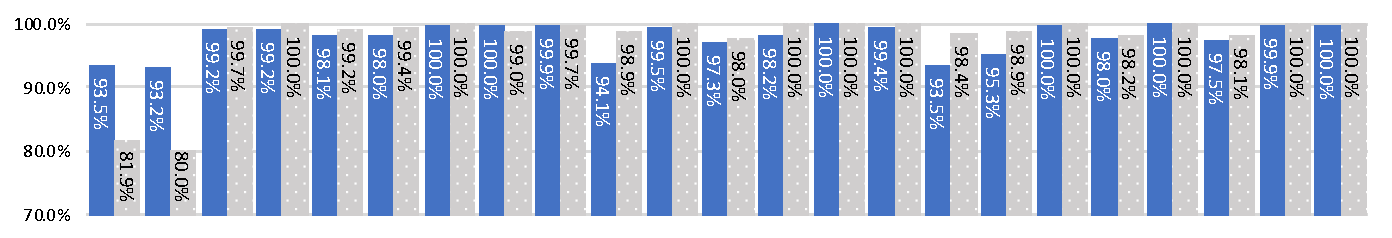
\includegraphics[width=\textwidth]{../img/plots/cog_canonical_baseline_no_labels.pdf}
	\end{subfigure}%
	\newline
	\begin{subfigure}{\textwidth}
		\centering
		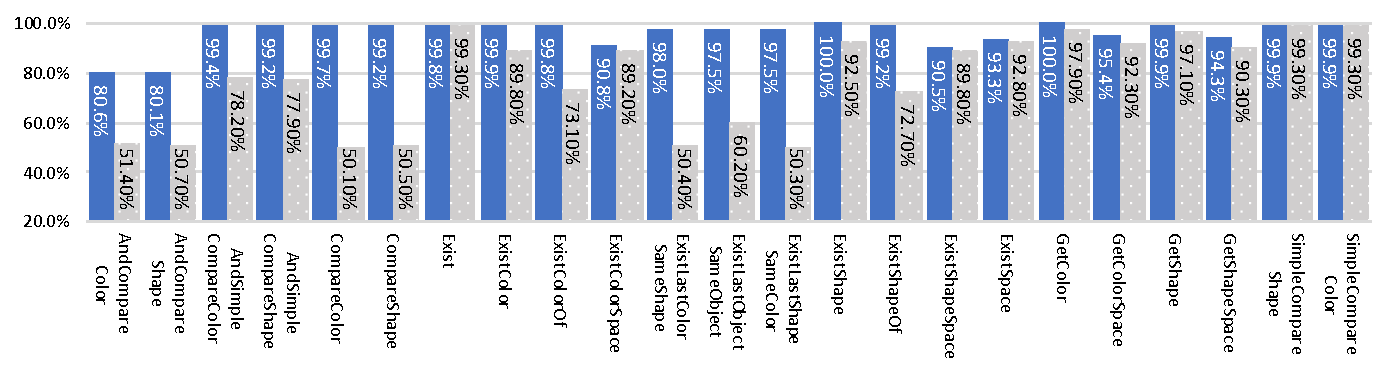
\includegraphics[width=\textwidth]{../img/plots/cog_hard_baseline_labels.pdf}
	\end{subfigure}%
	\caption{Comparison of test set accuracies of SAMNet (blue) with original results achieved by the baseline model~\cite{yang2018dataset} (dotted gray) on Canonical (top) and Hard (bottom) variants of the COG dataset.}
	\label{fig:samnet_cog_detailed}\vspace{-10pt}
\end{figure*}

\subsection{Performance of SAMNet on CLEVR}
\label{sec:clevr-baseline-compare}
CLEVR images contain objects characterized by a set of attributes (shape, color, size and material). The questions are grouped into 5 categories: \textit{Exist}, \textit{Count}, \textit{CompareInteger}, \textit{CompareAttribute}, \textit{QueryAttribute}.
The CLEVR authors also introduced CLEVR-CoGenT (Constrained Generalization Test), containing 2 variants, CoGenT-A and CoGenT-B, with varying combinations of color-shape attributes.
The colors are partitioned into two complementary families:
Gray, Blue, Brown, Yellow in Family A; and Red, Green, Purple, Cyan in Family B.
The cubes and cylinders take colors from complementary families in each variant with opposite configurations; the spheres can take any color in both variants (See~\cref{tab:cogent_conditions}).
As the input domain consist of the set of objects with all attribute values, both variants differ by their marginal distributions $P_S$ and $P_T$.

\cref{fig:clevr_baselines} presents the accuracy achieved by SAMNet when compared to selected state-of-the-art models, namely: Transparency by Design networks (TbD)~\cite{mascharka2018transparency}, Feature-wise Linear Modulation (FiLM)~\cite{perez2018film} and the Program Generator + Execution Engine (PG + EE)~\cite{johnson2017inferring}.
SAMNet reaches a comparable 96.2\% accuracy, with TbD achieving the best score of 98.7\%.


\subsection{Performance of SAMNet on COG}
\label{sec:cog-baseline-compare}

COG dataset contains short videos, with associated questions grouped into 23 categories\footnote{COG also proposes a pointing version of the tasks, which are not considered in this work.}.
COG comes in two variants: Canonical (easy) and Hard, differing mainly on the number of frames in the video, the maximum amount of look-back in frame history containing relevant information for reasoning, and the number of object distractors present in a given frame (see~\cref{tab:cog_variants}).
Since the number of task classes is large, we designed a 2-level hierarchy of task groups using the
description of tasks, as shown in~\cref{fig:task-groups}.

\begin{table}[htbp]
	\centering
	\begin{tabular}{lccc}
		\toprule
		Variant	& Frames & History	& Distractors \\
		\midrule
		Canonical (Easy) & 4 & 3 & 1\\
		Hard  & 8 & 7 & 10\\
		\bottomrule
	\end{tabular}
	\caption{Details of the Canonical and Hard variants of COG.}
	\label{tab:cog_variants}
\end{table}


\begin{figure}[b!]
	\centering
	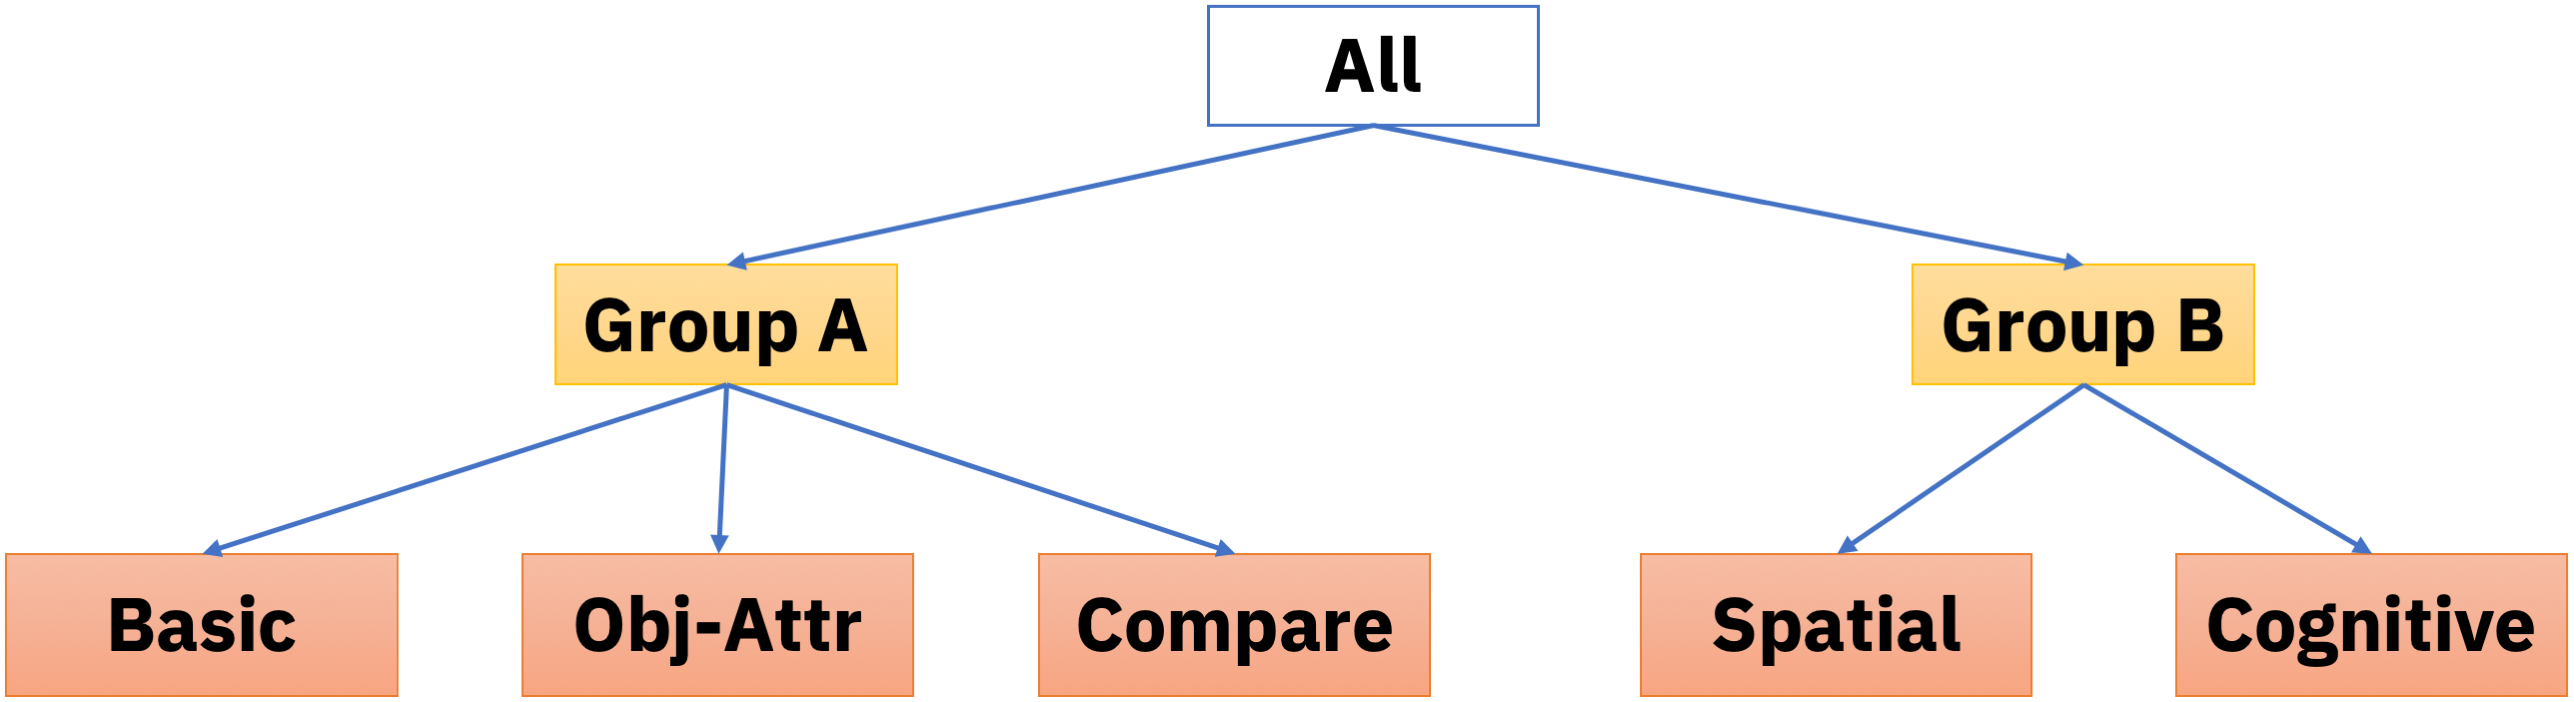
\includegraphics[width=0.5\textwidth]{../img/architecture/hierarchy}
	\caption{Hierarchy of Task Groups in the COG dataset.}
	\label{fig:task-groups}
\end{figure}



For groups at the lowest level, we chose the following task classes to be placed in those groups.
Below, substitute each of \textit{Shape} and \textit{Color} for  \uX{} to obtain the task class.
\begin{description}
	\item[Basic:] \textit{Exist}\uX, \textit{Get}\uX{} and \textit{Exist};
	\item[Obj-Attr:] \emph{SimpleCompare}\uX{} and \textit{AndSimpleCompare}\uX;
	\item[Compare:] \textit{Compare}\uX,  \textit{AndCompare}\uX{} \& \textit{Exist}\uX\textit{Of};
	\item[Spatial:] \textit{ExistSpace}, \textit{Exist}\uX\textit{Space}, and \textit{Get}\uX\textit{Space};
	\item[Cognitive:] \textit{ExistLastColorSameShape}, \textit{ExistLastShapeSameColor} and \textit{ExistLastObjectSameObject}
\end{description}


We compared our results with the baseline model introduced in in~\cite{yang2018dataset}, the same paper as the COG dataset.
The most important results are highlighted in~\cref{fig:samnet_cog_detailed}; full comparison can be found in the supplementary material.

For the Canonical variant (top row), we achieve similar accuracies for the majority of tasks (with a total average accuracy of 98.0\%, compared to 97.6\% for the baseline model), with significant improvements (around 13 points) for \textit{AndCompare} tasks.
As these tasks focus on compositional questions referring to two objects, we hypothesize that our model achieves better accuracy due to its ability to selectively pick and store relevant objects from the past frames in its external memory.
For the Hard variant, we achieve a total average accuracy of 96.1\% compared to 80.1\% for the baseline model, demonstrating that our model can adapt to larger number of frames and distractors.
SAMNet improves upon the baseline model on all tasks, with improvements varying from 0.5 to more than 30 points, especially outperforming in the most complex tasks (\textit{AndCompare}\uX, \textit{Compare}\uX).


\subsection{Feature transfer using CLEVR-CoGenT}
\label{sec:feature}

In order to quantify SAMNet's feature transfer ability, we used the CoGenT variants of CLEVR and performed a set of experiments, starting from training on CoGenT-A, followed by:
an immediate test (zero-shot learning) on CoGenT-B; and fine-tuning for a single epoch on 30k samples from CoGenT-B before testing (following the methodology used in~\cite{johnson2017inferring,mascharka2018transparency,perez2018film,marois2018transfer}).
In \cref{fig:CoGenT-B-results}, we compare the achieved performance with the previously selected state-of-the-art models.
We also consider a direct test on CoGenT-A; and a test on CoGenT-A after fine-tuning on B.

\begin{figure}[htbp]
	\centering
	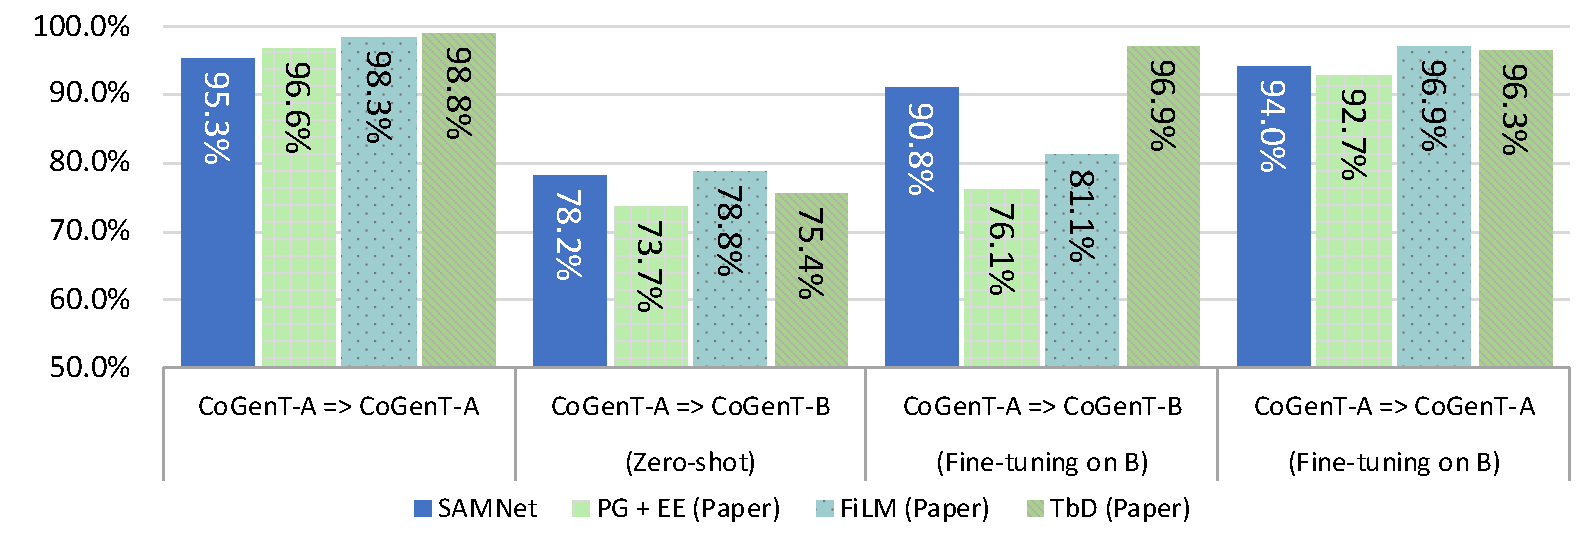
\includegraphics[width=\textwidth]{../img/plots/cogent_feature_transfer_baselines.pdf}
	\caption{Feature transfer: test accuracies when transferring between CoGenT-A and CoGenT-B.}
	\label{fig:CoGenT-B-results}
\end{figure}

When training and testing on CoGenT-A, SAMNet performs slightly worse than the other models, matching the results observed in \cref{sec:clevr-baseline-compare}.
When zero-shot testing on CoGenT-B, all models show relatively good performance (around 75\%), which represents nonetheless a drop of 17 points with respect to CoGenT-A.
All models perform better when fine-tuned on CoGenT-B.
However, this process also results in a degradation of performance on CoGenT-A, with SAMNet and TbD showing an ability to limit this drop in accuracy.
While this suggests both models were able to adapt representations for both domains, these representations are not fully disentangled.

\subsection{Temporal transfer in COG}
\label{sec:temporal}

Temporal transfer tests the transfer learning ability regarding the frame sequence length, frame history required for reasoning, and the number of distracting objects.
Therefore, we train the models on the Canonical variant of COG dataset and test them on the Hard variant~(\cref{fig:samnet_cog_overall_transfer}).
As the original paper~\cite{yang2018dataset} didn't provide such experiments, we supplement the original accuracies (denoted as gray-dotted) with the ones achieved by the COG baseline model that we have obtained by running the original code (gray-striped) provided by the authors~\cite{yang2018implement}.

\begin{figure}[htbp]
	\centering
	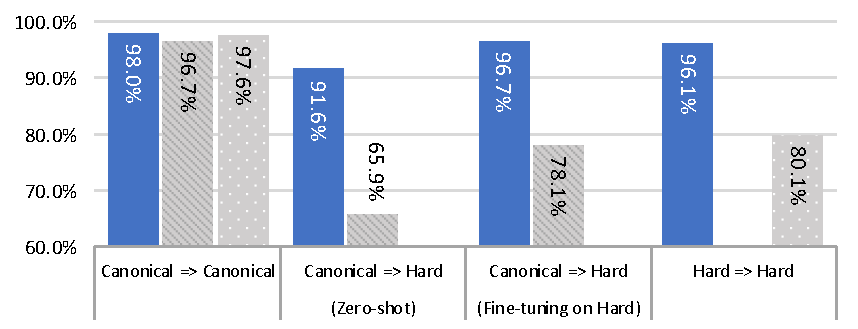
\includegraphics[width=0.8\textwidth]{../img/plots/cog_temporal_transfer_baselines.pdf}
	\caption{Temporal transfer capabilities of SAMNet (blue) and baseline models (gray -striped and -dotted) when moving from Canonical to Hard  in COG.}
	\label{fig:samnet_cog_overall_transfer}
\end{figure}

The first column displays the aggregated scores when training and testing on the Canonical variant.
The close scores of both base models (gray striped and dotted) highlight the faithful reproduction of the baseline model.
For both cases of zero-shot learning and fine-tuning using a single epoch, SAMNET significantly outperformed the baseline model, by 25 and 17 points respectively.
This might partially results from the frame-by-frame processing of videos executed by SAMNet by design, as opposed to the processing of aggregated frames performed by the baseline.
Interestingly, fine-tuning yields a mild boost of +0.6\% on the accuracy achieved by the model trained exclusively on the Hard variant.
This suggests that SAMNet managed to develop elementary skills (such as memory usage and attention on relevant entities) and successfully uses them when dealing with longer videos and more complex scenes.

%This suggest that it suffices to train SAMNet on simpler videos to enable learning of good memory usage and attention on relevant entities in order to achieve comparable, if not better, performance on longer video frames with more complex scenes.
